% mainfile: ../../main.tex
\chapter{Observations}\label{ch:exp:observations}
\AutoLettrine{Pidgeons}
\section{\Acrlong{tmm} simulations of the membrane structure}\label{sec:exp:tmm}
The \gls{tmm} is a computationally efficient method of obtaining the electric field in layered structures.
In this section, I perform simulations of the heterostructure membranes investigated in \thispart using the \package{PyMoosh} package~\cite{Langevin2024} to elucidate the observed quenching of \gls{pl} when illuminating gate electrodes as well as the overall optical efficiency.\sidenote{
    Strictly speaking, the term \acrshort{tmm} only refers to one of the several formalisms implemented in the \package{PyMoosh} package.
    While fast, it not the most numerically stable, and other methods may be preferred if wall time is not a limiting issue.
}
I will first briefly recap the simulation method following \citer{Langevin2024}.
For more details, refer to \ibid and references therein.

Consider a layered structure along $z$ with interfaces at $z_i, i\in\lbrace 0, 1, \dotsc, N+1\rbrace$ that is translationally invariant along $x$ and $y$.
Each layer $i$ may consist of a different dielectric material characterized by a (complex) relative permittivity $\epsilon_{r,i}$.\sidenote{
    We disregard magnetic materials with relative permeability $\mu_r\neq 1$ for simplicity.
}
The electric field component along $y$ of an electromagnetic wave \gls{te} mode originating in some far away point satisfies the Helmholtz equation
\begin{equation}\label{eq:exp:tmm:helmholtz}
    \pdv[2]{E_y}{z} + \gamma_i^2 E_y = 0,
\end{equation}
where $\gamma_i = \sqrt{\epsilon_{r,i}k_0^2 - k_x^2}$ with $k_0=\flatfrac{\omega}{c}$ the wave vector in vacuum and $k_x$ the component along $x$.
In layer $i$ of the structure, the solution to \cref{eq:exp:tmm:helmholtz} may be written as a superposition of plane waves incident and reflected on the lower and upper interfaces,
\begin{equation}
    \begin{dcases}
        E_{y,i}(z) = A_i^{+}\exp{\i\gamma_i(z-z_{i})} + B_i^{+}\exp{-\i\gamma_i(z-z_{i})}, \\
        E_{y,i}(z) = A_i^{-}\exp{\i\gamma_i(z-z_{i+1})} + B_i^{-}\exp{-\i\gamma_i(z-z_{i+1})},
    \end{dcases}
\end{equation}
where the coefficients with superscript $+$ ($-$) are referenced to the phase at the upper (lower) interface, respectively.
Matching these solutions at $z=z_i$ for all $i$ to satisfy the interface conditions imposed by Maxwell's equations gives rise to a linear system of equations, the solution to which can be obtained through several different methods.

A particularly simple method is the \acrlong{tmm} ($T$-matrix formalism), which corresponds to writing the interface conditions at $z=z_i$ as the matrix equation
\begin{equation}\label{eq:exp:tmm:interface}
    \pmqty{A_{i+1}^{+}\\B_{i+1}^{+}} = T_{i,i+1}\pmqty{A_{i}^{-}\\B_{i}^{-}}
\end{equation}
with
\begin{equation}\label{eq:exp:tmm:T}
    T_{i,i+1} = \frac{1}{2\gamma_{i+1}}\begin{pmatrix}
        \gamma_{i} + \gamma_{i+1} & \gamma_{i} - \gamma_{i+1} \\
        \gamma_{i} - \gamma_{i+1} & \gamma_{i} + \gamma_{i+1}
    \end{pmatrix}
\end{equation}
the transfer matrix for interface $i$.
Connecting the coefficients for adjacent interfaces within a layer of height $h_i = z_{i+1} - z_{i}$ requires propagating the phase,
\begin{equation}\label{eq:exp:tmm:propagation}
    \pmqty{A_{i}^{-}\\B_{i}^{-}} = C_{i}\pmqty{A_{i}^{+}\\B_{i}^{+}},
\end{equation}
with
\begin{equation}\label{eq:exp:tmm:C}
    C_{i} = \exp{\diag(-\i\gamma_i h_i, \i\gamma_i h_i)}.
\end{equation}
Iterating \cref{eq:exp:tmm:C,eq:exp:tmm:T}, the total transfer matrix $T = T_{0,N+1}$ then reduces to the matrix product
\begin{equation}\label{eq:exp:tmm:T:total}
    T = T_{N,N+1}\prod_{i=0}^{N-1} T_{i,i+1} C_i.
\end{equation}
From $T$, the reflection and transmission coefficients can be obtained as $r=A_0^{-}=-\flatfrac{T_{01}}{T_{00}}$ and $t=B_{N+1}^{+}=rT_{10} + T_{11}$.
Taking the absolute value square of reflection and transmission coefficients then yields the reflectance \reflectance and the transmittance \transmittance, which correspond to the fraction of total incident power being reflected and transmitted, respectively.
To obtain the absorptance \absorptance, the fraction of power being absorbed, in layer $i$, one can compute the difference of the $z$-components of the Poynting vectors (\cf \cref{eq:setup:optics:coupling:poynting}) at the top of layers $i$ and $i+1$.
In the \gls{te} case considered here, \cref{eq:setup:optics:coupling:poynting} reduces to
\begin{equation}
    \bvec{S}_i = \re\left[\frac{\gamma_i^{\ast}}{\gamma_0}\left(A_i^{+} - B_i^{+}\right)^{\ast}\left(A_i^{+} + B_i^{+}\right)\right]
\end{equation}
and is hence straightforward to extract from the calculation of either the $S$ or $T$ matrices.

\Cref{eq:exp:tmm:T:total} is simple to evaluate on a computer, making this method attractive for numerical applications.
However, the opposite signs in the argument of the exponentials in \cref{eq:exp:tmm:C} can lead to instabilities for evanescent waves ($\gamma_i\in\mathbb{C}$) due to finite-precision floating point arithmetic~\cite{Duetz}.
Rewriting \cref{eq:exp:tmm:T} to have incoming and outgoing fields on opposite sides of the equality alleviates this issue while sacrificing the simple matrix-multiplication composition rule in what is known as the scattering matrix ($S$-matrix) formalism.

Beyond the calculation of the aforementioned coefficients, the \gls{tmm} formalism also allows to compute the full spatial dependence of the fields.
Two cases are implemented in \package{PyMoosh}; first, irradiation of the layered structured with a Gaussian beam rather than plane waves of infinite extent, and second, a current line source inside the structure.

\begin{figure}
    \centering
    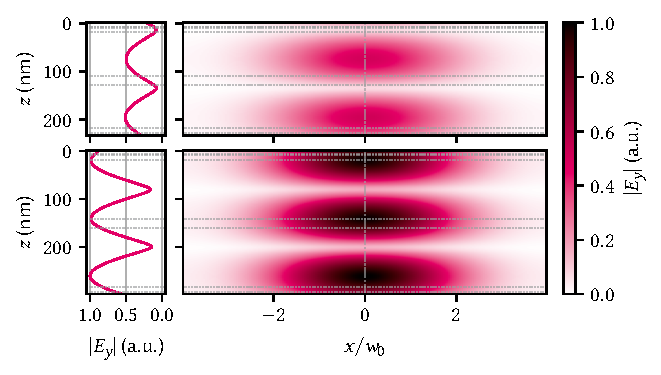
\includegraphics{img/pdf/experiment/tmm_field}
    \caption[\imgsource{img/py/experiment/tmm.py}]{}
    \label{fig:exp:tmm:field}
\end{figure}

\begin{marginfigure}
    \centering
    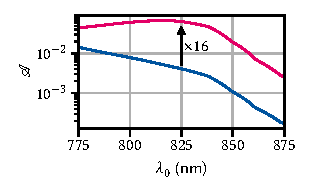
\includegraphics{img/pdf/experiment/tmm_absorptance}
    \caption[\imgsource{img/py/experiment/tmm.py}]{}
    \label{fig:exp:tmm:wavelengths}
\end{marginfigure}

\begin{marginfigure}
    \centering
    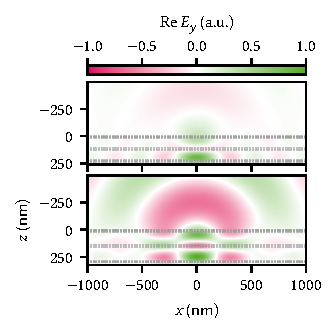
\includegraphics{img/pdf/experiment/tmm_green_opt_tgbg}
    \caption[\imgsource{img/py/experiment/tmm.py}]{}
    \label{fig:exp:tmm:green:opt:tgbg}
\end{marginfigure}

\begin{marginfigure}
    \centering
    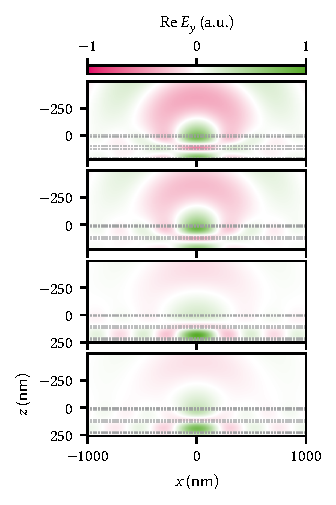
\includegraphics{img/pdf/experiment/tmm_green}
    \caption[\imgsource{img/py/experiment/tmm.py}]{}
    \label{fig:exp:tmm:green}
\end{marginfigure}

